\chapter[Results and Evaluation Status]{Results, Reproducibility, and Evaluation Status}
\label{ch:results}

\section{Purpose of this chapter}
This chapter distinguishes executable evidence from legacy illustrative material. Performance values are reported only when they are generated by the repository's evaluation script and accompanied by a split-integrity assessment. This distinction is essential because an image-level split can produce optimistic estimates when scans or views from the same subject occur in more than one partition.

\section{Current cohort audit}
The validated loader uses repaired BrEaST and OASBUD subject-level partitions, containing 302 training, 63 validation, and 62 test images. The audit reports no cross-partition subjects in either dataset. BUSI remains excluded because its generated \texttt{sample\_} filenames prevent verification of patient-level separation from the local files alone.

\section{Executable checkpoint result}
The fresh EfficientNet-B0 checkpoint was evaluated with the shared preprocessing implementation on the repaired test partition. Table~\ref{tab:provisional_result} is generated from that execution and describes local-cohort research evidence, not clinical or external validation.

\begin{table}[htbp]
\centering
\caption{EfficientNet-B0 result on the audited 62-image BrEaST and OASBUD test partition.}
\label{tab:provisional_result}
\begin{tabular}{@{}lccccc@{}}
\toprule
\textbf{Model} & \textbf{Samples} & \textbf{Accuracy} & \textbf{Macro F1} & \textbf{Macro Recall} & \textbf{ROC-AUC} \\ \midrule
EfficientNet-B0 & 62 & 67.74\% & 0.6774 & 0.6803 & 0.7419 \\ \bottomrule
\end{tabular}
\end{table}

At class level, the benign class (33 images) had precision 0.72, recall 0.64, and F1 0.68. The malignant class (29 images) had precision 0.64, recall 0.72, and F1 0.68. These values describe this held-out local cohort and do not establish external or clinical performance.

\begin{table}[htbp]
\centering
\caption{Class-level results at the fixed 0.5 malignant-probability threshold.}
\label{tab:class_metrics}
\begin{tabular}{@{}lrrrr@{}}
\toprule
\textbf{True class} & \textbf{Support} & \textbf{Precision} & \textbf{Recall} & \textbf{F1} \\
\midrule
Benign & 33 & 0.7241 & 0.6364 & 0.6774 \\
Malignant & 29 & 0.6364 & 0.7241 & 0.6774 \\
\bottomrule
\end{tabular}
\end{table}

The confusion matrix in Figure~\ref{fig:provisional_confusion} contains 21 correctly classified benign images, 21 correctly classified malignant images, 12 benign images classified as malignant, and 8 malignant images classified as benign. Figure~\ref{fig:provisional_roc} plots the corresponding threshold sweep. Both figures are generated by \texttt{evaluate.py} from the same prediction run as Table~\ref{tab:provisional_result}.

\begin{figure}[htbp]
    \centering
    
\includegraphics[width=0.72\textwidth]{figures/fig2_confusion_matrix.png}
    \caption{Confusion matrix for the EfficientNet-B0 checkpoint on the audited 62-image test partition. Local-cohort research evidence only.}
    \label{fig:provisional_confusion}
\end{figure}

The stored probabilities also support threshold-sensitive analysis without fitting the model again. Figure~\ref{fig:discrimination_calibration} combines a malignant-class precision-recall curve with a five-bin reliability diagram. Average precision is 0.6803, compared with a malignant prevalence of 0.4677. The Brier score is 0.2144 and the evaluator's expected calibration error is 0.0652. These are descriptive test-set diagnostics. No probability calibration or threshold selection was fitted on the test data.

\begin{figure}[htbp]
    \centering
    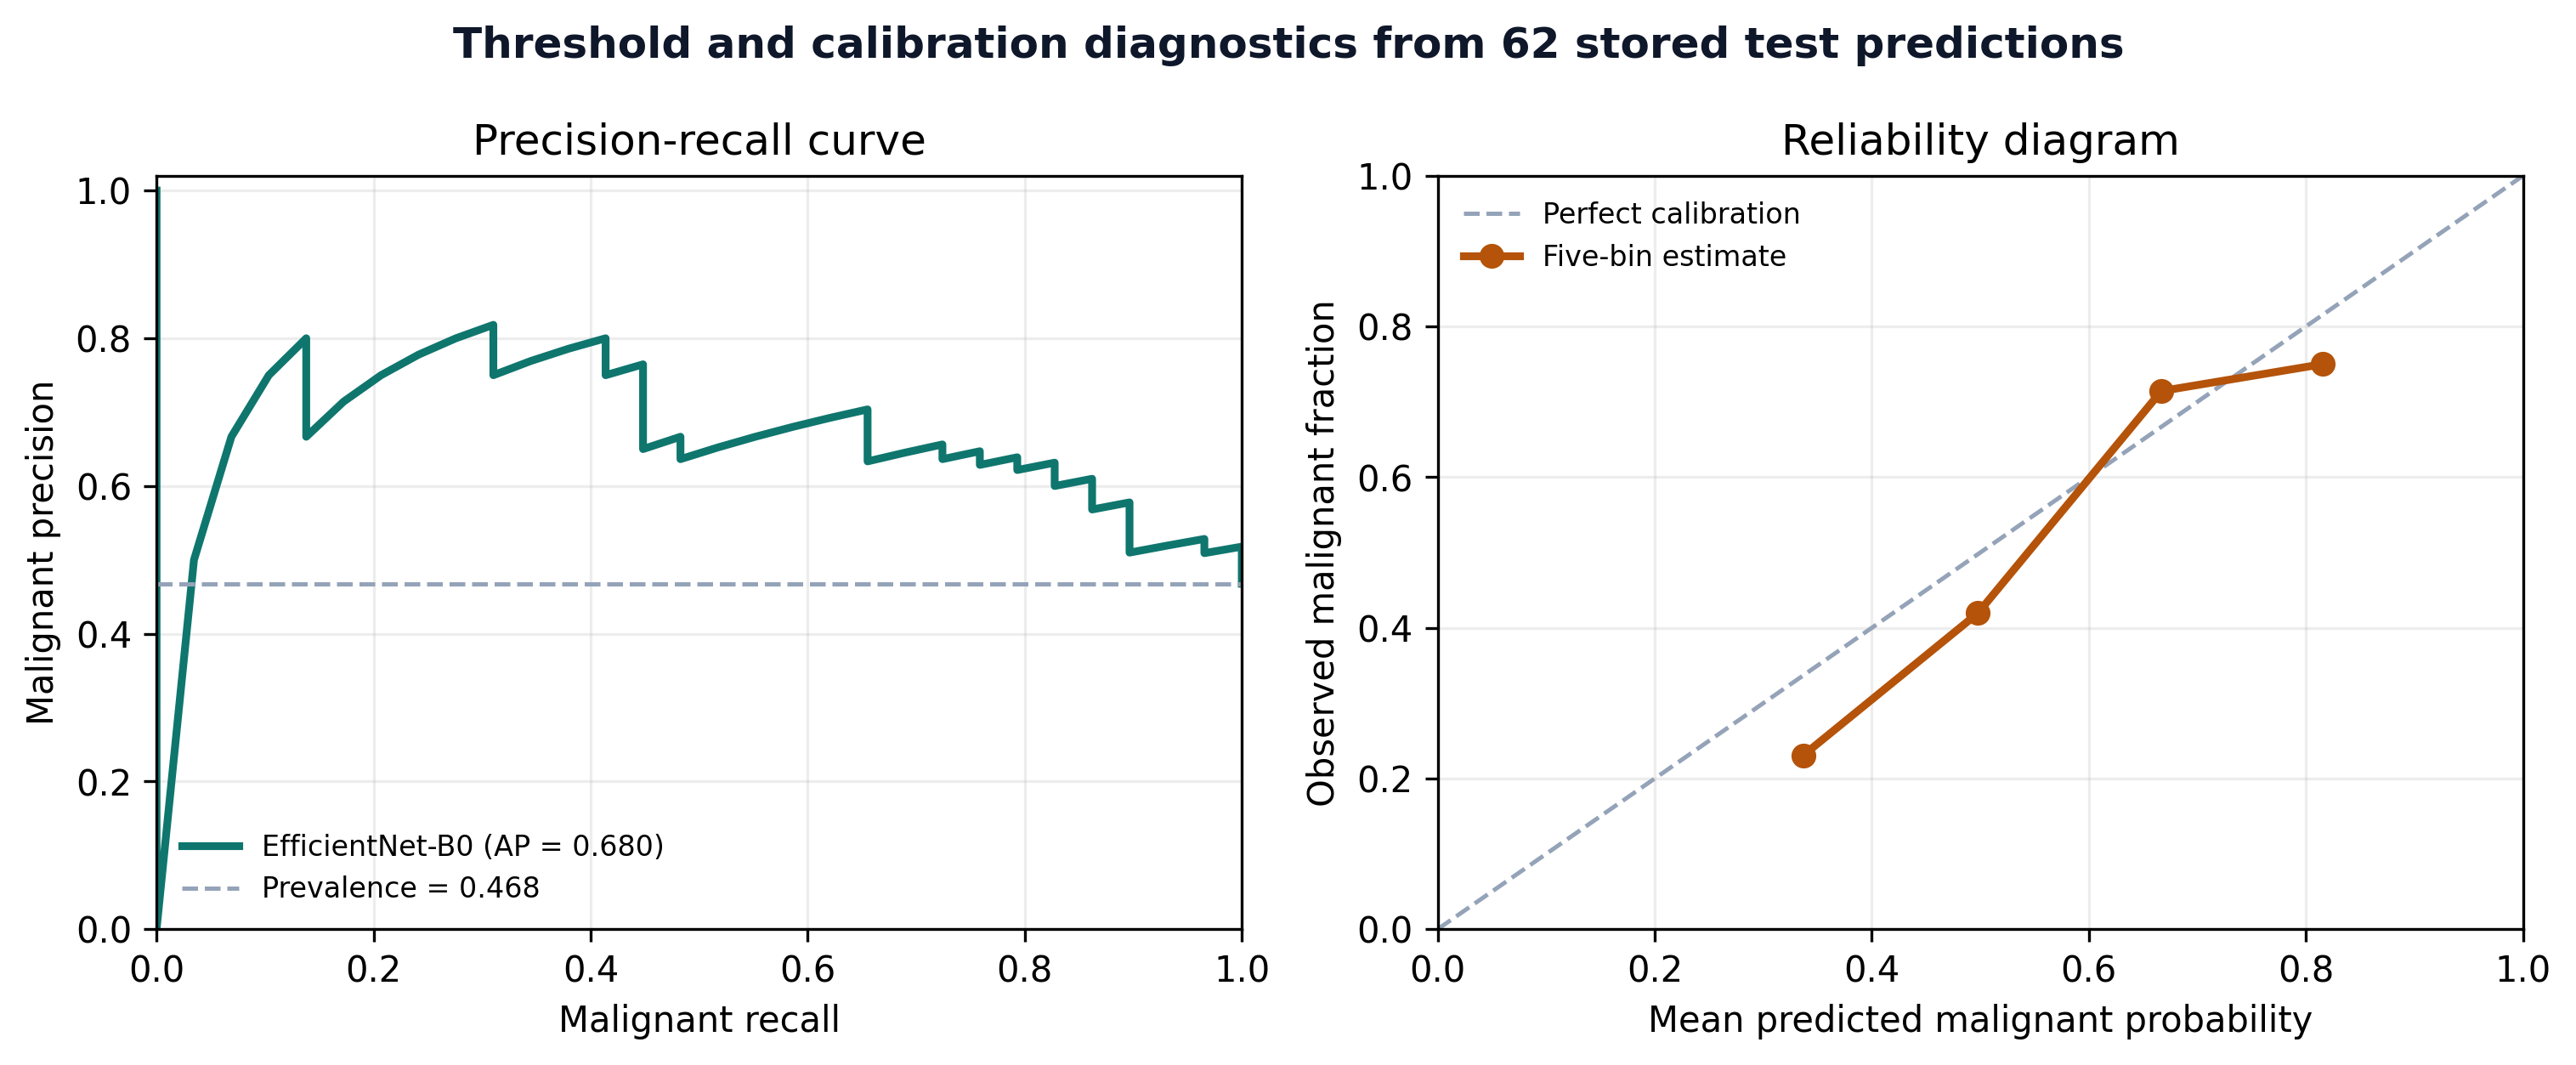
\includegraphics[width=0.98\textwidth]{figures/fig12_discrimination_calibration.png}
    \caption{Precision-recall and reliability views derived from the 62 stored EfficientNet-B0 predictions. Average precision summarises malignant-class ranking, while the reliability panel compares mean predicted probability with the observed fraction in five bins. The small number of cases makes each point uncertain.}
    \label{fig:discrimination_calibration}
\end{figure}

\begin{figure}[htbp]
    \centering
    
\includegraphics[width=0.72\textwidth]{figures/fig3_roc_curve.png}
    \caption{ROC curve for the same 62-image audited evaluation run (ROC-AUC 0.7419).}
    \label{fig:provisional_roc}
\end{figure}

\section{Withdrawn legacy figures and tables}
Earlier project assets contained fixed benchmark values, simulated pseudo-labelling tables, and illustrative noise trajectories. They are not used as results because they were not regenerated from stored model predictions on an audited cohort. The superseded files have been removed from the submission-facing figures and archived with an explicit warning; they must not be cited as measured performance.

\section{Additional evidence figures}
The notebook contains the same confusion matrix and ROC curve included above. Three additional figures were generated from the notebook's machine-readable evidence files rather than drawn by hand. Figure~\ref{fig:dataset_composition} shows the class composition of the two audited datasets across the three partitions. BrEaST contributes 229 images and OASBUD contributes 198; the test split contains 62 images in total. The figure also makes the normal category visible in the training and validation folders, even though the current binary output contract maps it to the non-malignant side of the task.

\begin{figure}[htbp]
    \centering
    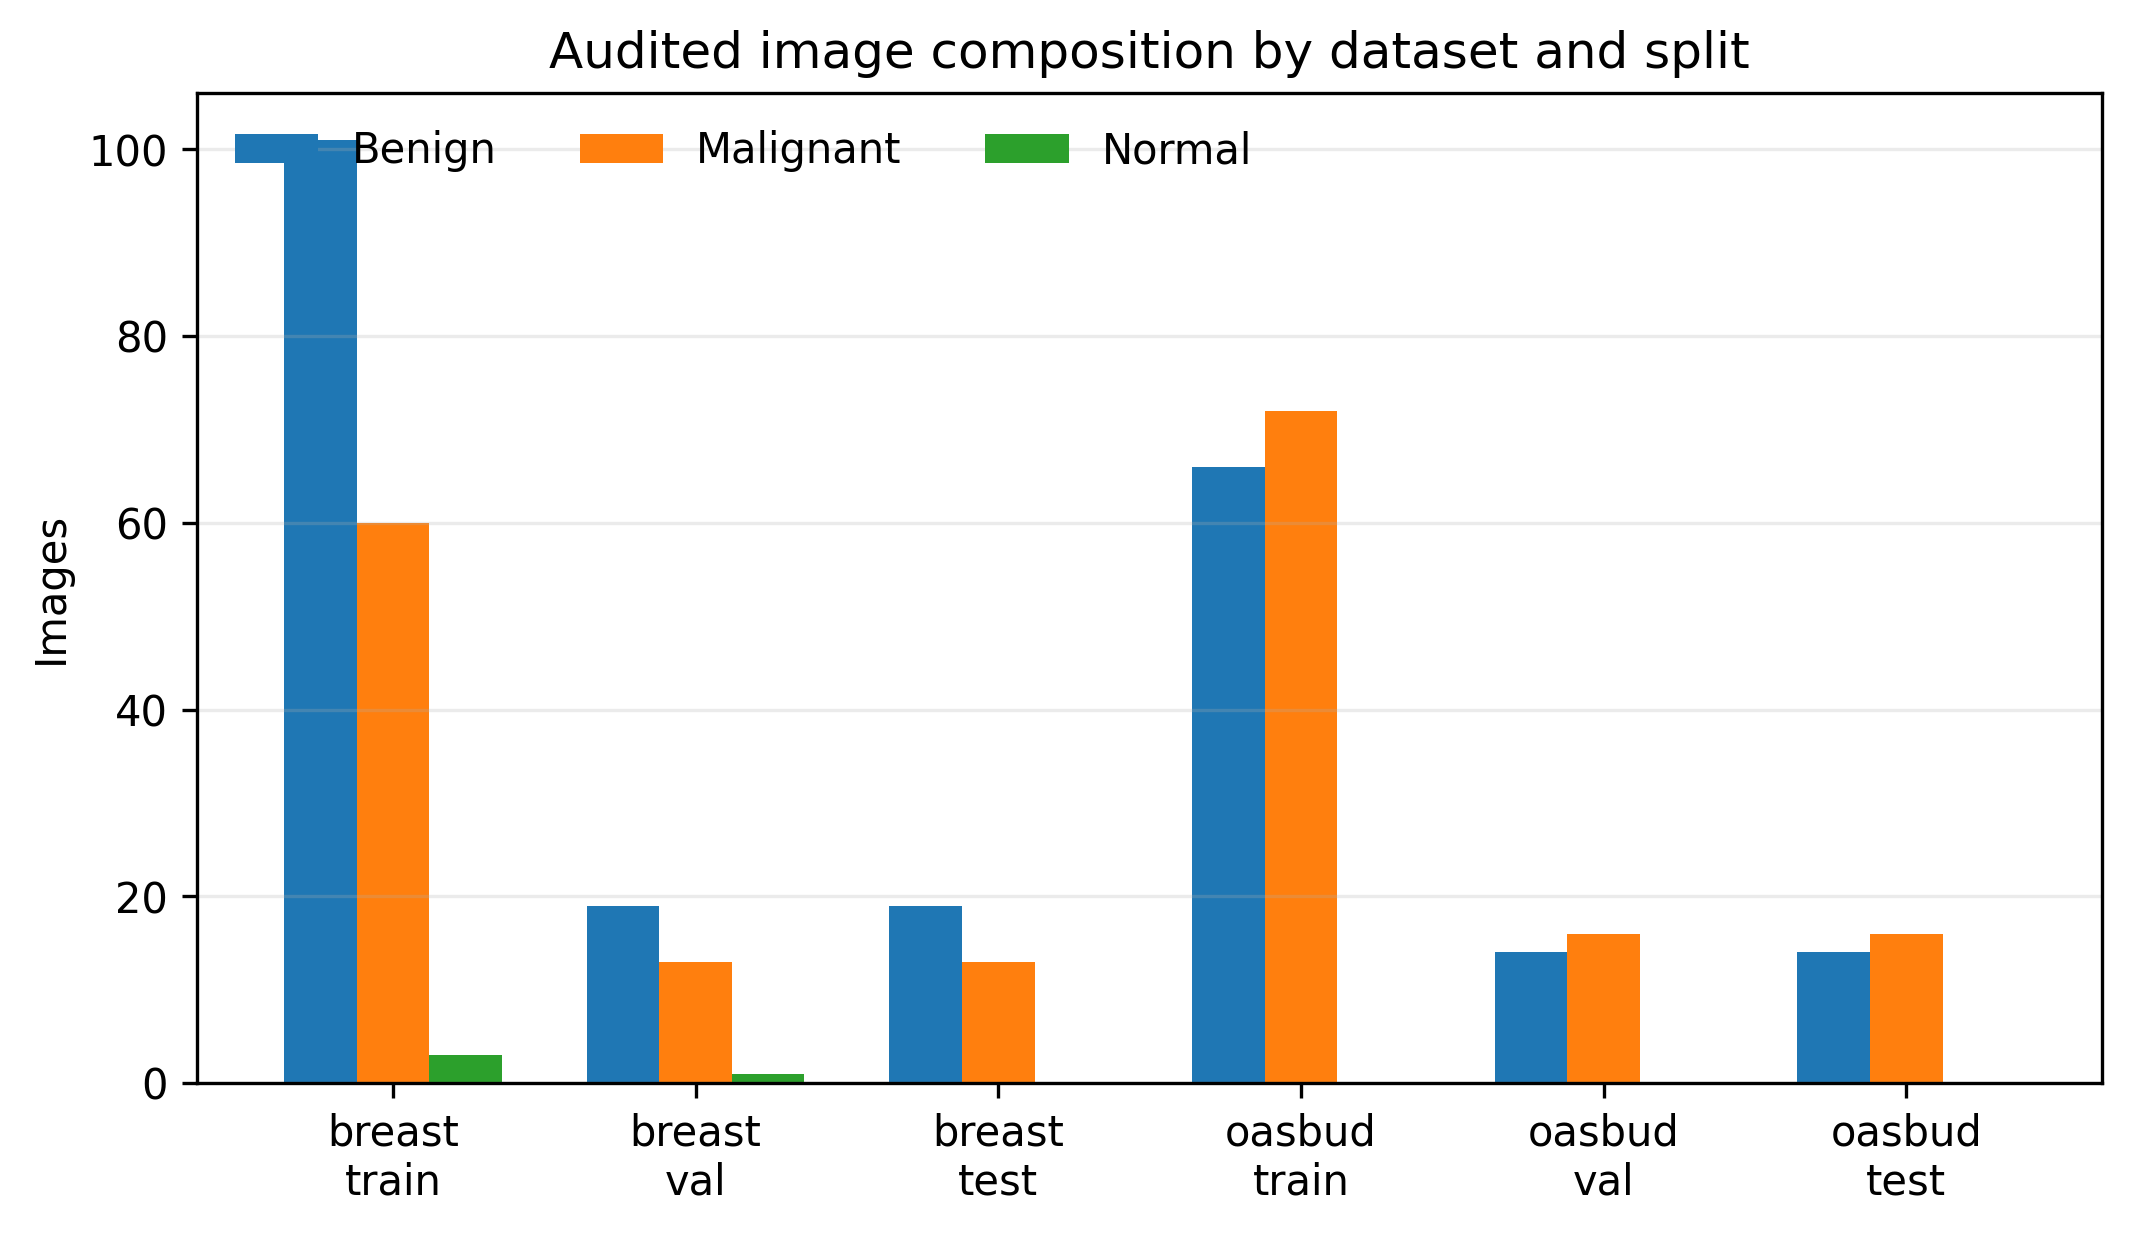
\includegraphics[width=0.88\textwidth]{figures/fig4_dataset_composition.png}
    \caption{Class composition of the audited BrEaST and OASBUD folders. Counts are read from the split audit; BUSI is excluded from the validated run.}
    \label{fig:dataset_composition}
\end{figure}

Figure~\ref{fig:model_benchmark} compares the three architectures under the same local test protocol. EfficientNet-B0 has the highest point estimates for accuracy, macro F1, and ROC-AUC in this run. The figure should be read as an internal benchmark, not as a comparison with published external systems. The common split and evaluator make the comparison useful for deciding what to investigate next, while the sample size limits the strength of any ranking claim.

\begin{figure}[htbp]
    \centering
    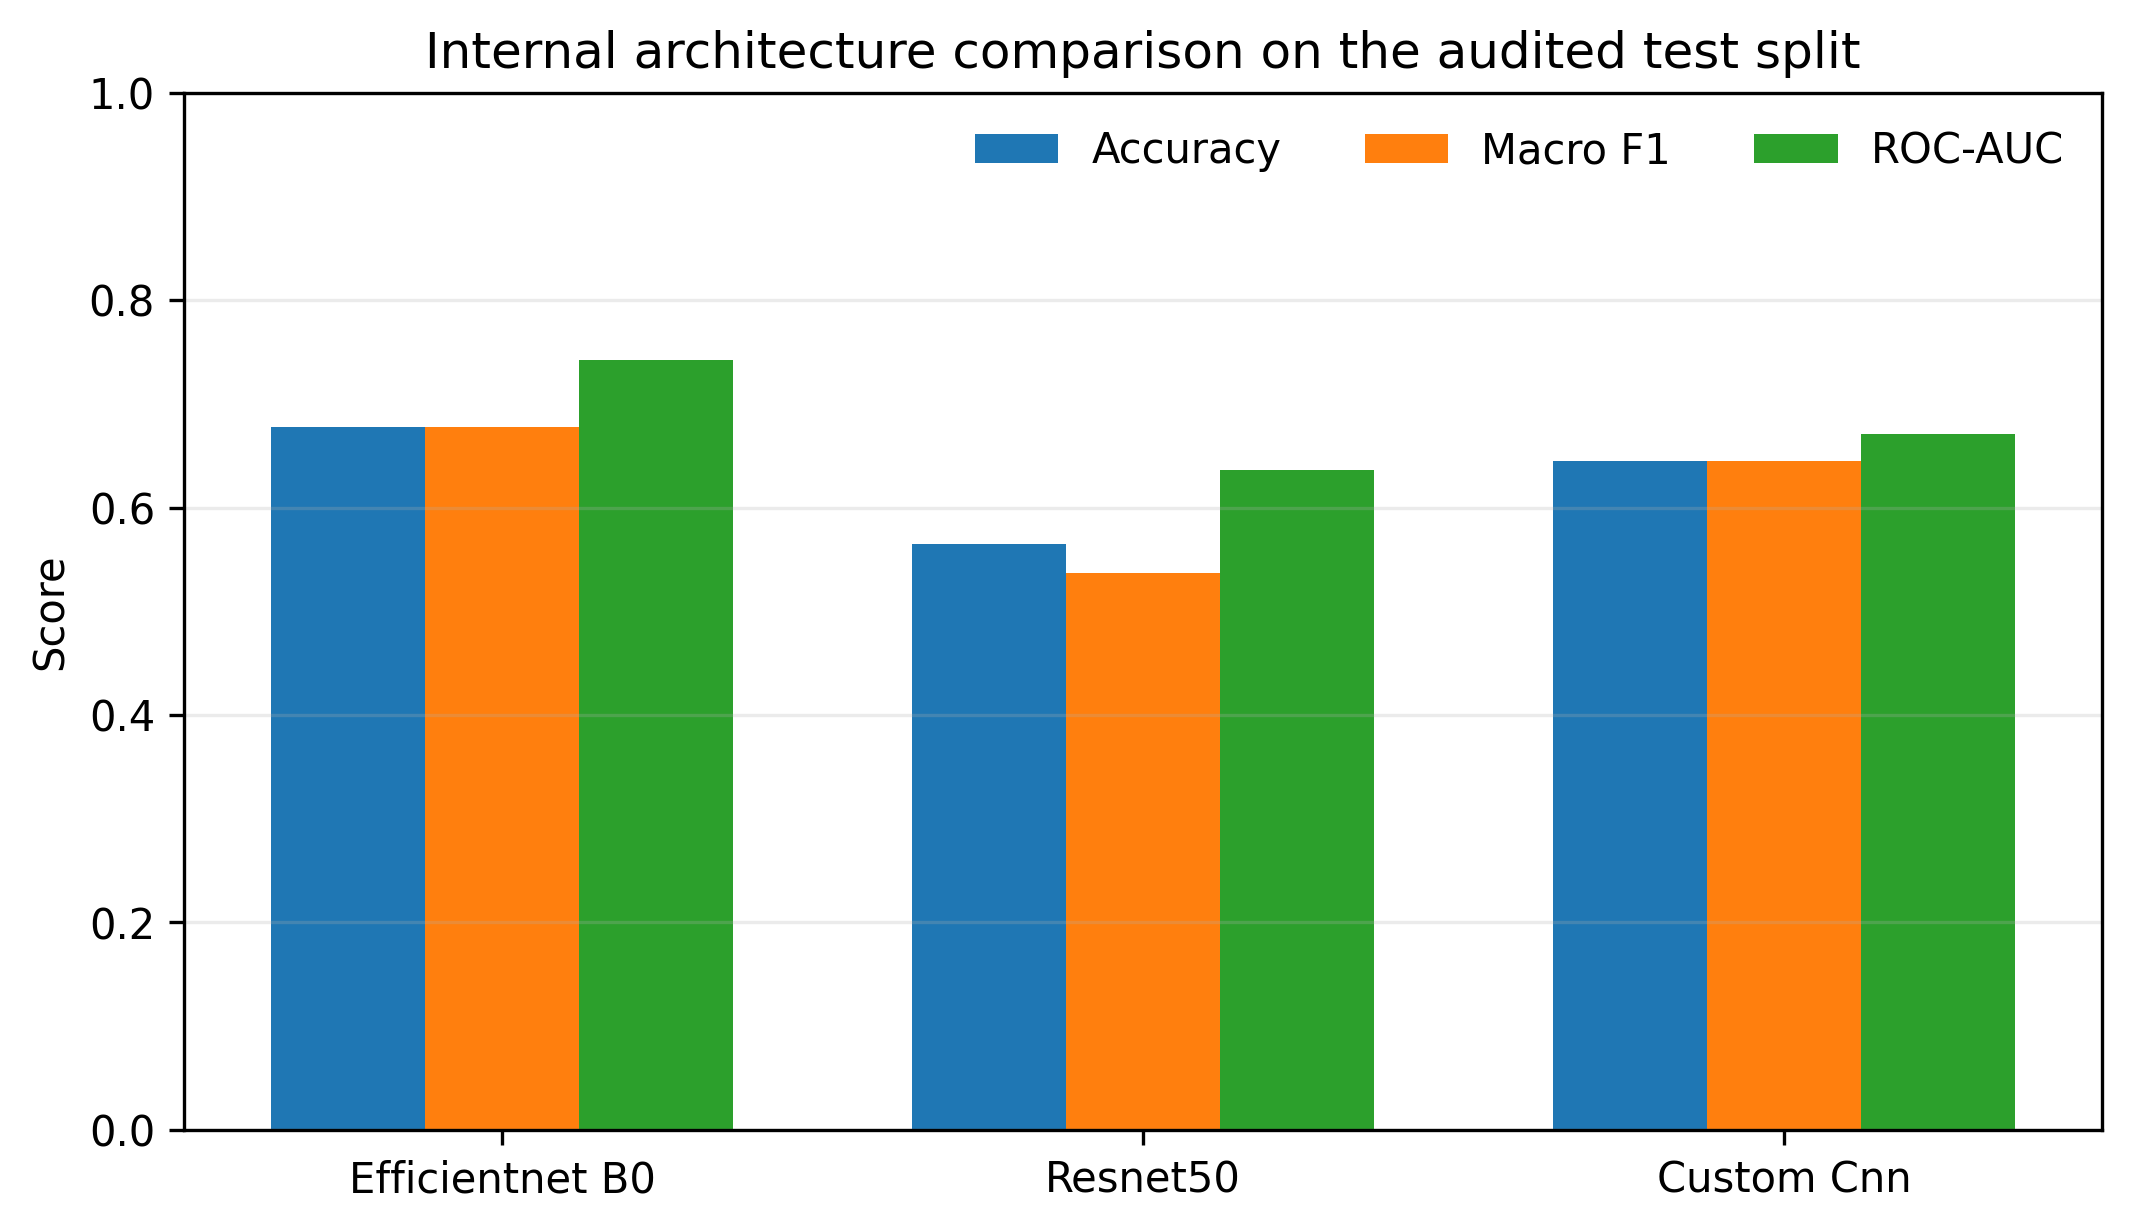
\includegraphics[width=0.88\textwidth]{figures/fig5_model_benchmark.png}
    \caption{Internal same-split comparison of the implemented model families. Scores are generated from the stored benchmark JSON.}
    \label{fig:model_benchmark}
\end{figure}

Figure~\ref{fig:accuracy_intervals} places the accuracy values beside their bootstrap intervals. The intervals overlap substantially, so the point-estimate ordering should not be treated as evidence that EfficientNet-B0 is superior in the wider population. This is a useful scientific finding in its own right: the current data support a baseline and a protocol, while a larger subject-level cohort is needed to resolve model differences.

\begin{figure}[htbp]
    \centering
    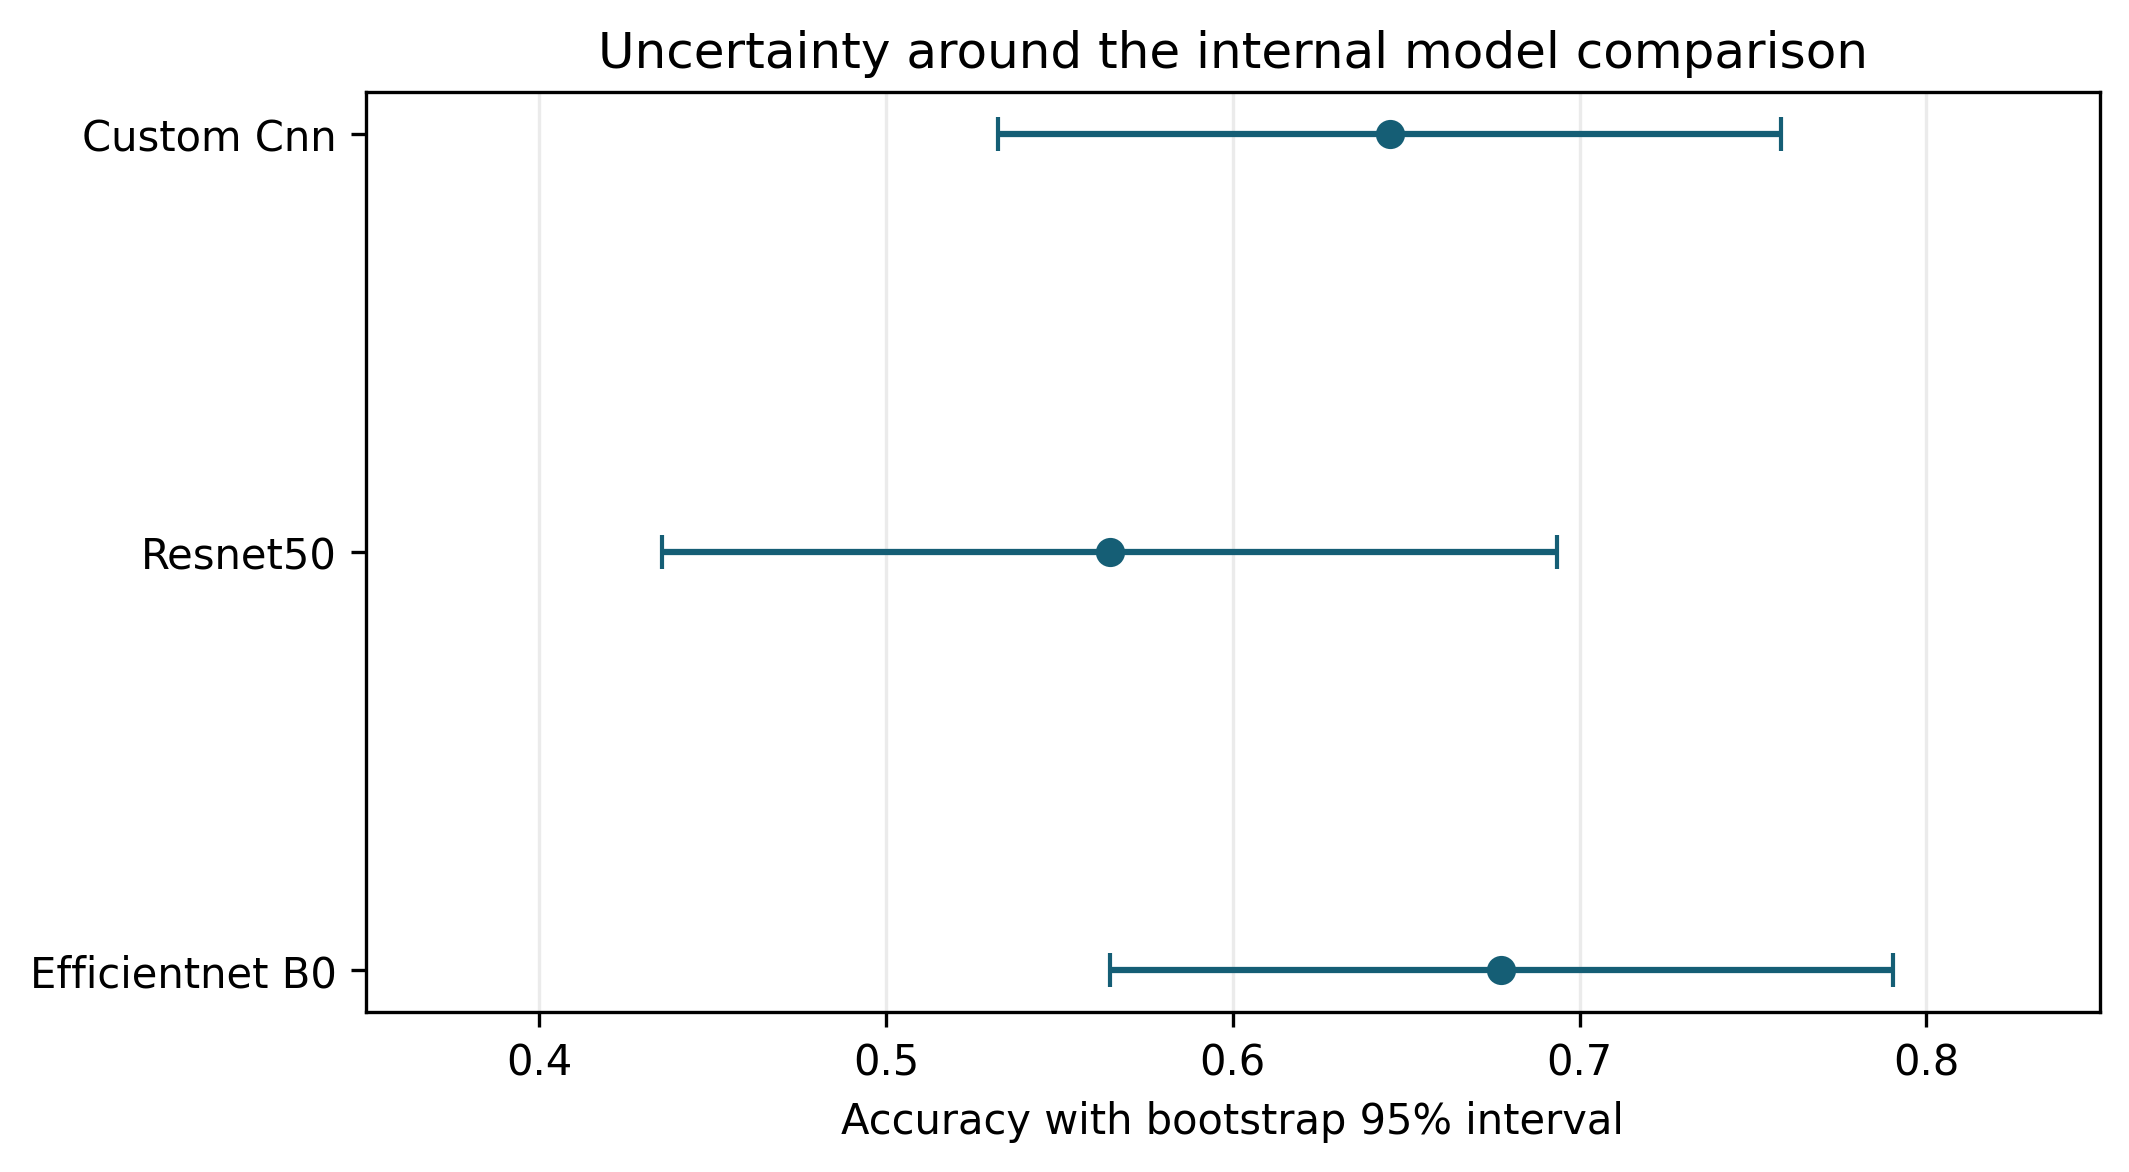
\includegraphics[width=0.88\textwidth]{figures/fig6_accuracy_intervals.png}
    \caption{Accuracy point estimates and bootstrap 95\% intervals for the internal model comparison.}
    \label{fig:accuracy_intervals}
\end{figure}

Together, the figures show why the report presents the model as a research baseline. The audited class counts are small, the classes are not perfectly balanced, and the uncertainty intervals are wide. The evidence supports further experimentation with restored provenance and multi-seed evaluation rather than a claim of diagnostic readiness.

\section{Final evaluation protocol}
The final study must assign every subject, including all views and masks, to exactly one partition. It should preserve a versioned manifest with source identifiers, label, split, checksum, preprocessing configuration, random seed, checkpoint hash, and per-image prediction. Accuracy, sensitivity, specificity, ROC-AUC, precision--recall AUC, calibration, and confidence intervals should then be calculated once on an untouched test partition. Noise and preprocessing ablations require separate trained/evaluated runs rather than manually specified curves.

\section{Interpretation}
The present evidence supports the implementation of a reproducible experimental framework, not superiority of a particular architecture or preprocessing method. The results should therefore be interpreted as a baseline engineering validation. Claims of clinical robustness, optimal pseudo-labelling thresholds, or state-of-the-art diagnostic performance are deferred pending the audited experiments described above.

\section{Internal model comparison}
The same evaluator compared the three implemented architectures on the same audited test partition. EfficientNet-B0 produced the strongest point estimates in this local run, followed by the custom CNN and then ResNet-50. This ordering is descriptive only. It is based on 62 test images, uses one training seed, and does not include a multi-seed uncertainty analysis for the architecture ranking.

\begin{table}[htbp]
\centering
\caption{Internal comparison on the same audited 62-image test partition. Parentheses give bootstrap 95\% intervals.}
\label{tab:model_comparison}
\scriptsize
\begin{tabular}{@{}lccc@{}}
\toprule
\textbf{Model} & \textbf{Accuracy} & \textbf{Macro F1} & \textbf{ROC-AUC} \\
\midrule
EfficientNet-B0 & 0.6774 (0.5645, 0.7903) & 0.6774 (0.5589, 0.7889) & 0.7419 (0.6217, 0.8616) \\
Custom CNN & 0.6452 (0.5323, 0.7581) & 0.6452 (0.5171, 0.7575) & 0.6708 (0.5330, 0.7979) \\
ResNet-50 & 0.5645 (0.4355, 0.6935) & 0.5374 (0.4038, 0.6649) & 0.6364 (0.5054, 0.7701) \\
\bottomrule
\end{tabular}
\end{table}

The comparison illustrates why a single accuracy value is insufficient. The EfficientNet result has a ROC-AUC of 0.7419, indicating useful ranking behaviour in this sample, but the score does not identify a clinically appropriate threshold. The custom CNN is higher than ResNet-50 on all three listed point estimates in this run. That observation is worth reporting, but it is not a scientific breakthrough: both models were tested on the same 62-image partition, each comparison represents one training seed, and every pair of bootstrap intervals overlaps. The comparison file retains only per-model summaries rather than paired predictions, so a paired test such as McNemar's test cannot be reconstructed. A significance claim would be unsupported. The observed differences may reflect capacity, optimisation, or random variation.

\section{Training-record limitation}

The three checkpoints preserve the selected epoch and validation summary, but not the complete epoch-by-epoch history. Table~\ref{tab:checkpoint_selection} reports everything that can be recovered. A learning curve cannot be reconstructed from one selected point, so no synthetic curve is included.

\begin{table}[htbp]
\centering
\caption{Checkpoint selection metadata retained by the completed runs.}
\label{tab:checkpoint_selection}
\begin{tabular}{@{}lrrr@{}}
\toprule
\textbf{Model} & \textbf{Selected epoch} & \textbf{Validation loss} & \textbf{Validation accuracy} \\
\midrule
EfficientNet-B0 & 5 & 0.6107 & 0.6667 \\
Custom CNN & 3 & 0.6431 & 0.6349 \\
ResNet-50 & 2 & 0.6662 & 0.6349 \\
\bottomrule
\end{tabular}
\end{table}

The training program now writes loss, accuracy, and learning rate after every epoch for future runs and embeds the history available at each best checkpoint. This change improves the next experiment without retraining or altering the evidence reported here.

\section{Uncertainty and calibration}
For the EfficientNet checkpoint, the bootstrap 95\% interval for accuracy was [0.5645, 0.7903], for macro F1 [0.5589, 0.7889], and for ROC-AUC [0.6217, 0.8616]. The expected calibration error was 0.0652 under the evaluator's binning procedure. These values make the result more informative than a point estimate alone, while still leaving substantial uncertainty. The interval width is a direct reminder that a small test set cannot support fine-grained claims about superiority.

Calibration should be separated from abstention in the web application. The API can hide low-margin outputs behind an ``UNCERTAIN'' display label, but that rule does not recalibrate the underlying probabilities. The reliability diagram in Figure~\ref{fig:discrimination_calibration} is an evaluation of the saved test predictions, not a fitted recalibration model. Temperature scaling or another calibration method would need to be fitted on validation data and checked once on an untouched test set. Until then, probabilities are useful for ranking and inspection, not for estimating a patient's probability of disease \citep{Guo2017}.

\section{What the errors show}
The EfficientNet confusion matrix contains eight malignant images classified as benign and twelve benign images classified as malignant. The two error directions are not interchangeable in a clinical setting, but the current study does not contain the clinical information needed to assign different costs or choose an operating point. It is therefore safer to report both class-wise recalls than to describe the model as simply accurate or safe.

Each mistaken image should be reviewed alongside its original file, processed crop, mask status, probability, and dataset source. Reviewers can ask whether the error is associated with an absent mask, a small lesion, a particular acquisition style, a label ambiguity, or an artefact at the image boundary. Such observations can generate hypotheses for the next experiment, but they should not be converted into causal explanations from visual inspection alone.

Figure~\ref{fig:prediction_examples} adds an image-level view of the stored predictions. The examples are selected by a fixed rule from \path{outputs/predictions.csv}: the lowest-probability correct benign case, the highest-probability correct malignant case, the highest-probability false positive, and the lowest-probability false negative. Each panel uses the same mask-guided crop and CLAHE path as evaluation. Green frames mark correct classifications and red frames mark errors.

\begin{figure}[htbp]
    \centering
    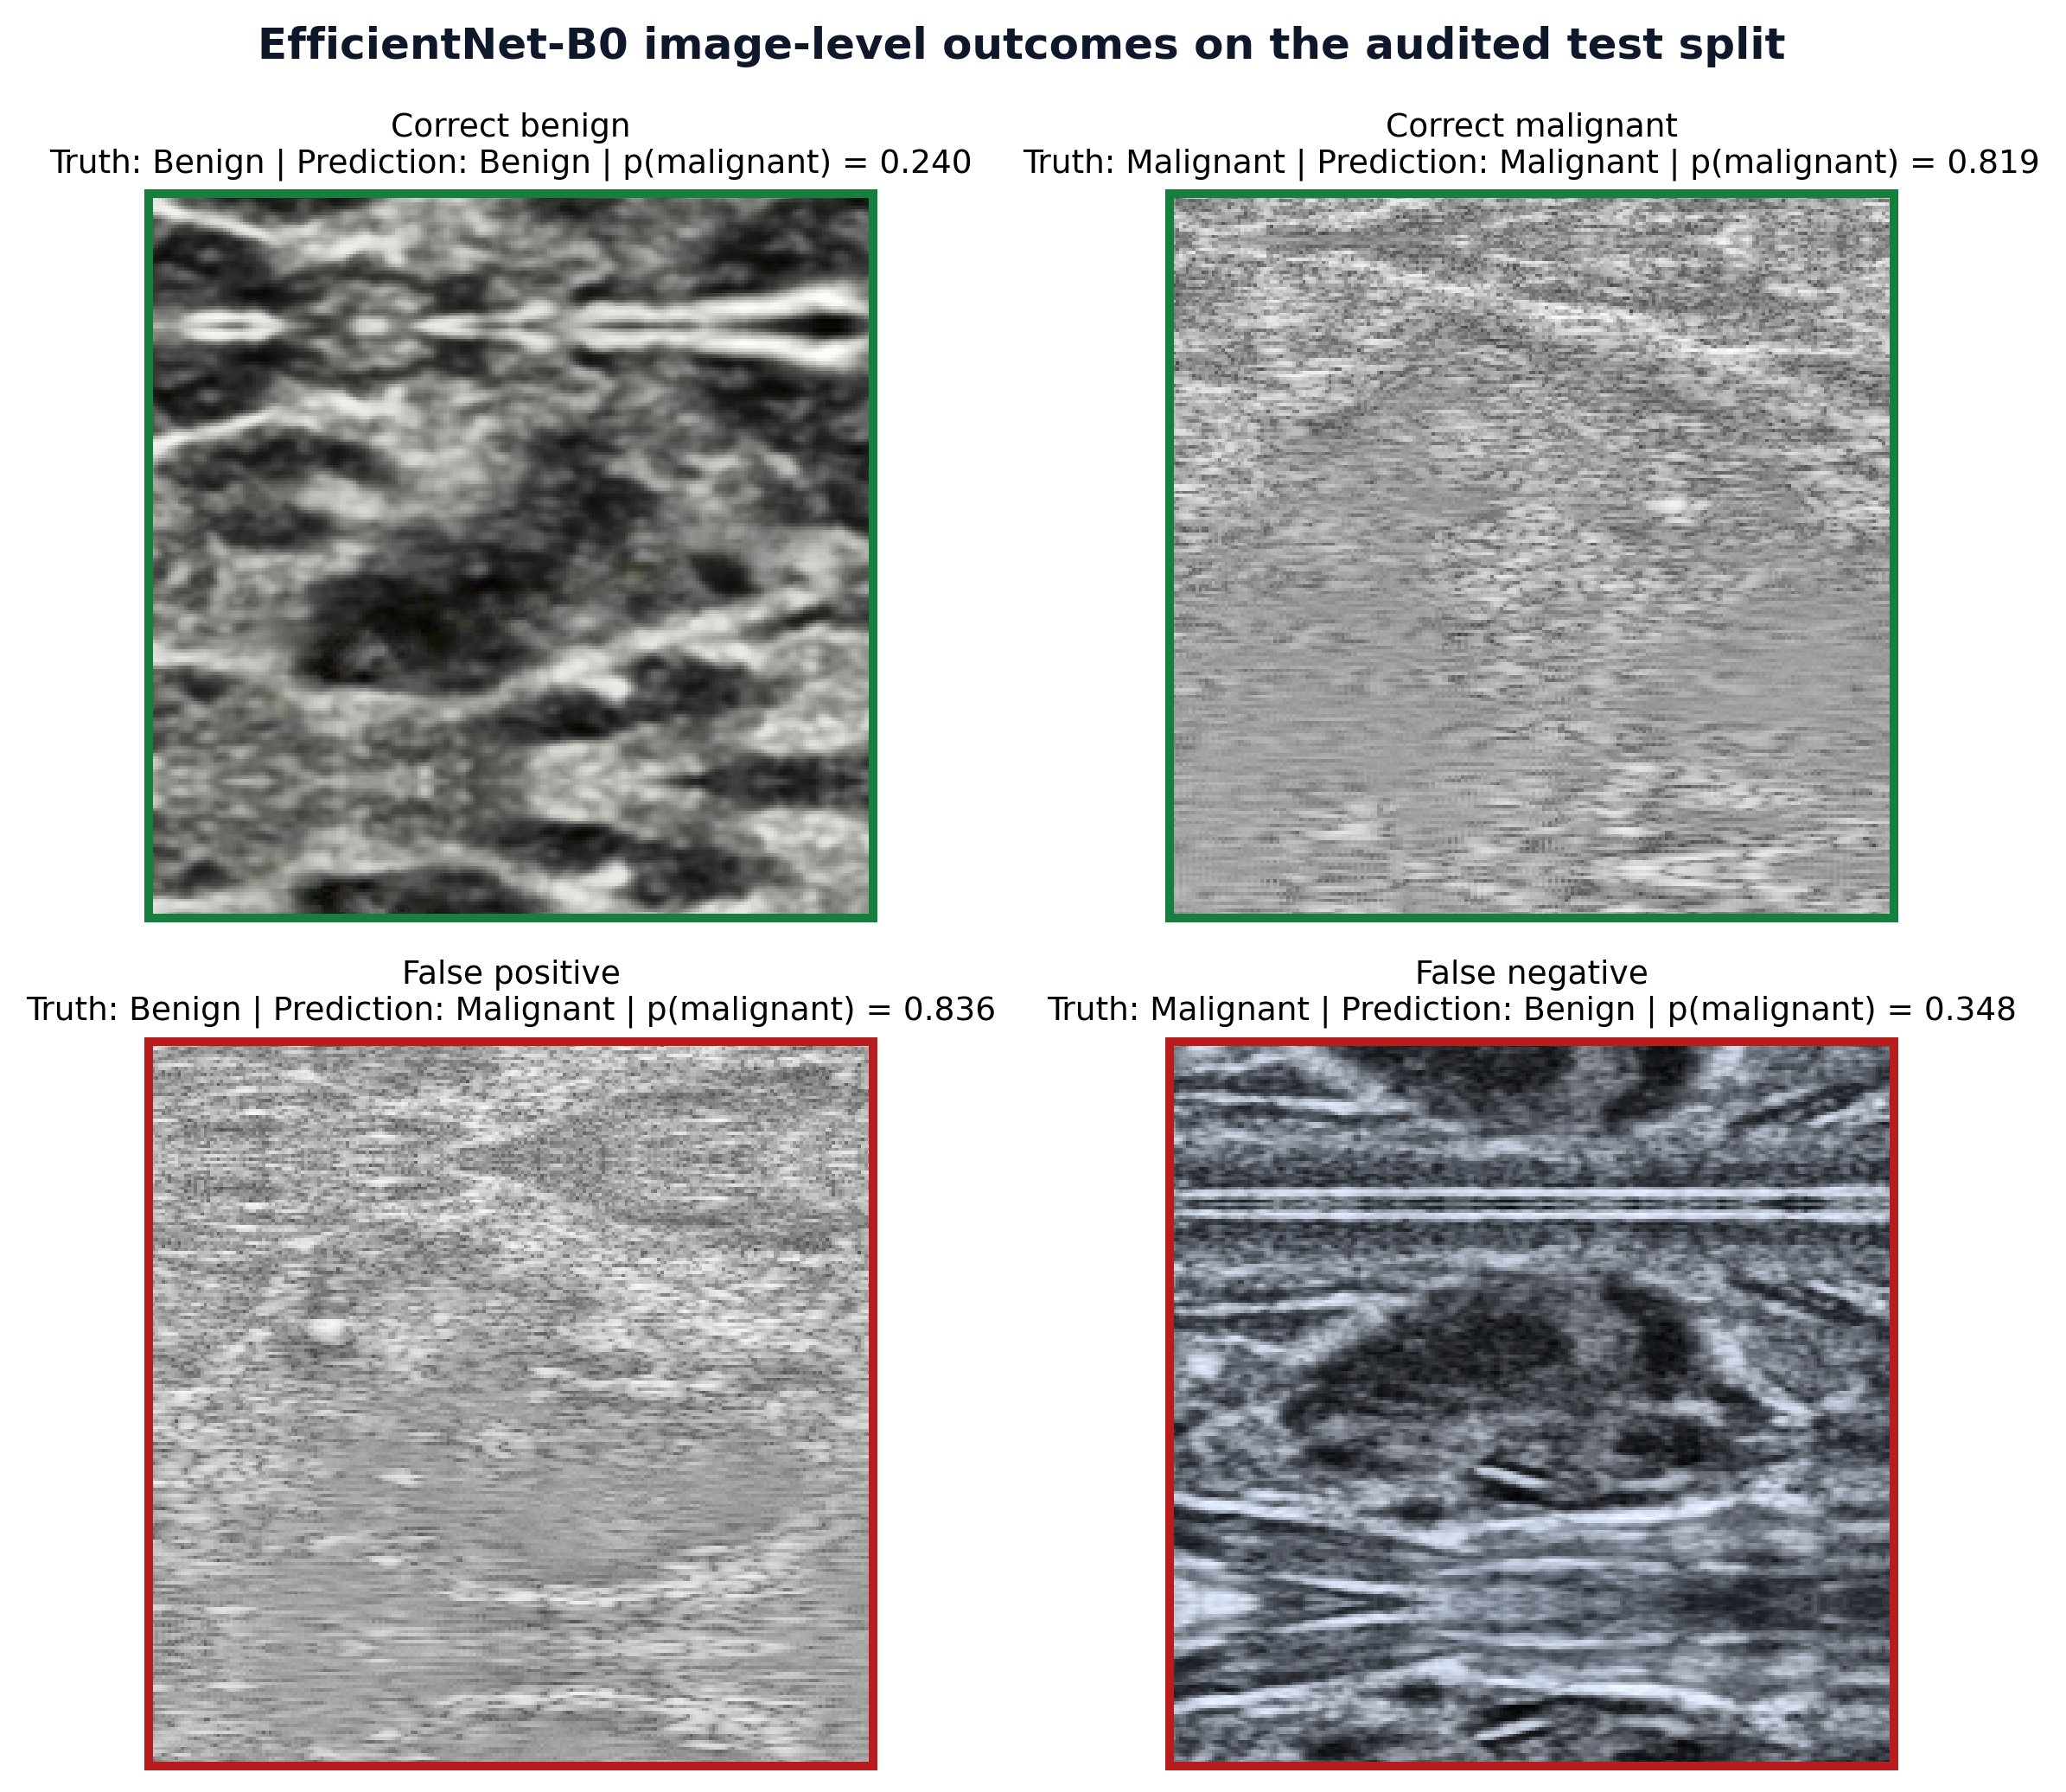
\includegraphics[width=0.88\textwidth]{figures/fig10_prediction_examples.png}
    \caption{Deterministically selected correct and incorrect EfficientNet-B0 outputs from the audited test partition. Panel headings report the true label, predicted label, and stored malignant-class probability. Visual inspection supports error analysis but does not establish the clinical reason for a decision.}
    \label{fig:prediction_examples}
\end{figure}

The false positive comes from OASBUD and the false negative from BrEaST, so the two displayed errors also span the distinct visual styles seen in Figure~\ref{fig:dataset_quality_examples}. That pattern is useful for planning a source-stratified analysis. Four selected images cannot show whether one dataset is systematically harder, and the error causes remain unresolved without a larger sample and expert review.

The full per-image table allows a source-level check. Table~\ref{tab:source_results} and Figure~\ref{fig:source_results} show that performance differs markedly between the two local sources. On BrEaST, accuracy was 0.7813 and specificity 0.8947. On OASBUD, accuracy was 0.5667 and specificity 0.2857, while malignant recall was higher at 0.8125. This pattern is compatible with source-dependent acquisition or reconstruction effects, but the sample is too small to identify a cause.

\begin{table}[htbp]
\centering
\caption{Source-stratified EfficientNet-B0 test results at the fixed 0.5 threshold.}
\label{tab:source_results}
\small
\begin{tabular}{@{}lrrrrrr@{}}
\toprule
\textbf{Source} & \textbf{$n$} & \textbf{Accuracy} & \textbf{Malignant recall} & \textbf{Specificity} & \textbf{ROC-AUC} & \textbf{AP} \\
\midrule
BrEaST & 32 & 0.7813 & 0.6154 & 0.8947 & 0.8259 & 0.7840 \\
OASBUD & 30 & 0.5667 & 0.8125 & 0.2857 & 0.6786 & 0.6853 \\
\bottomrule
\end{tabular}
\end{table}

\begin{figure}[htbp]
    \centering
    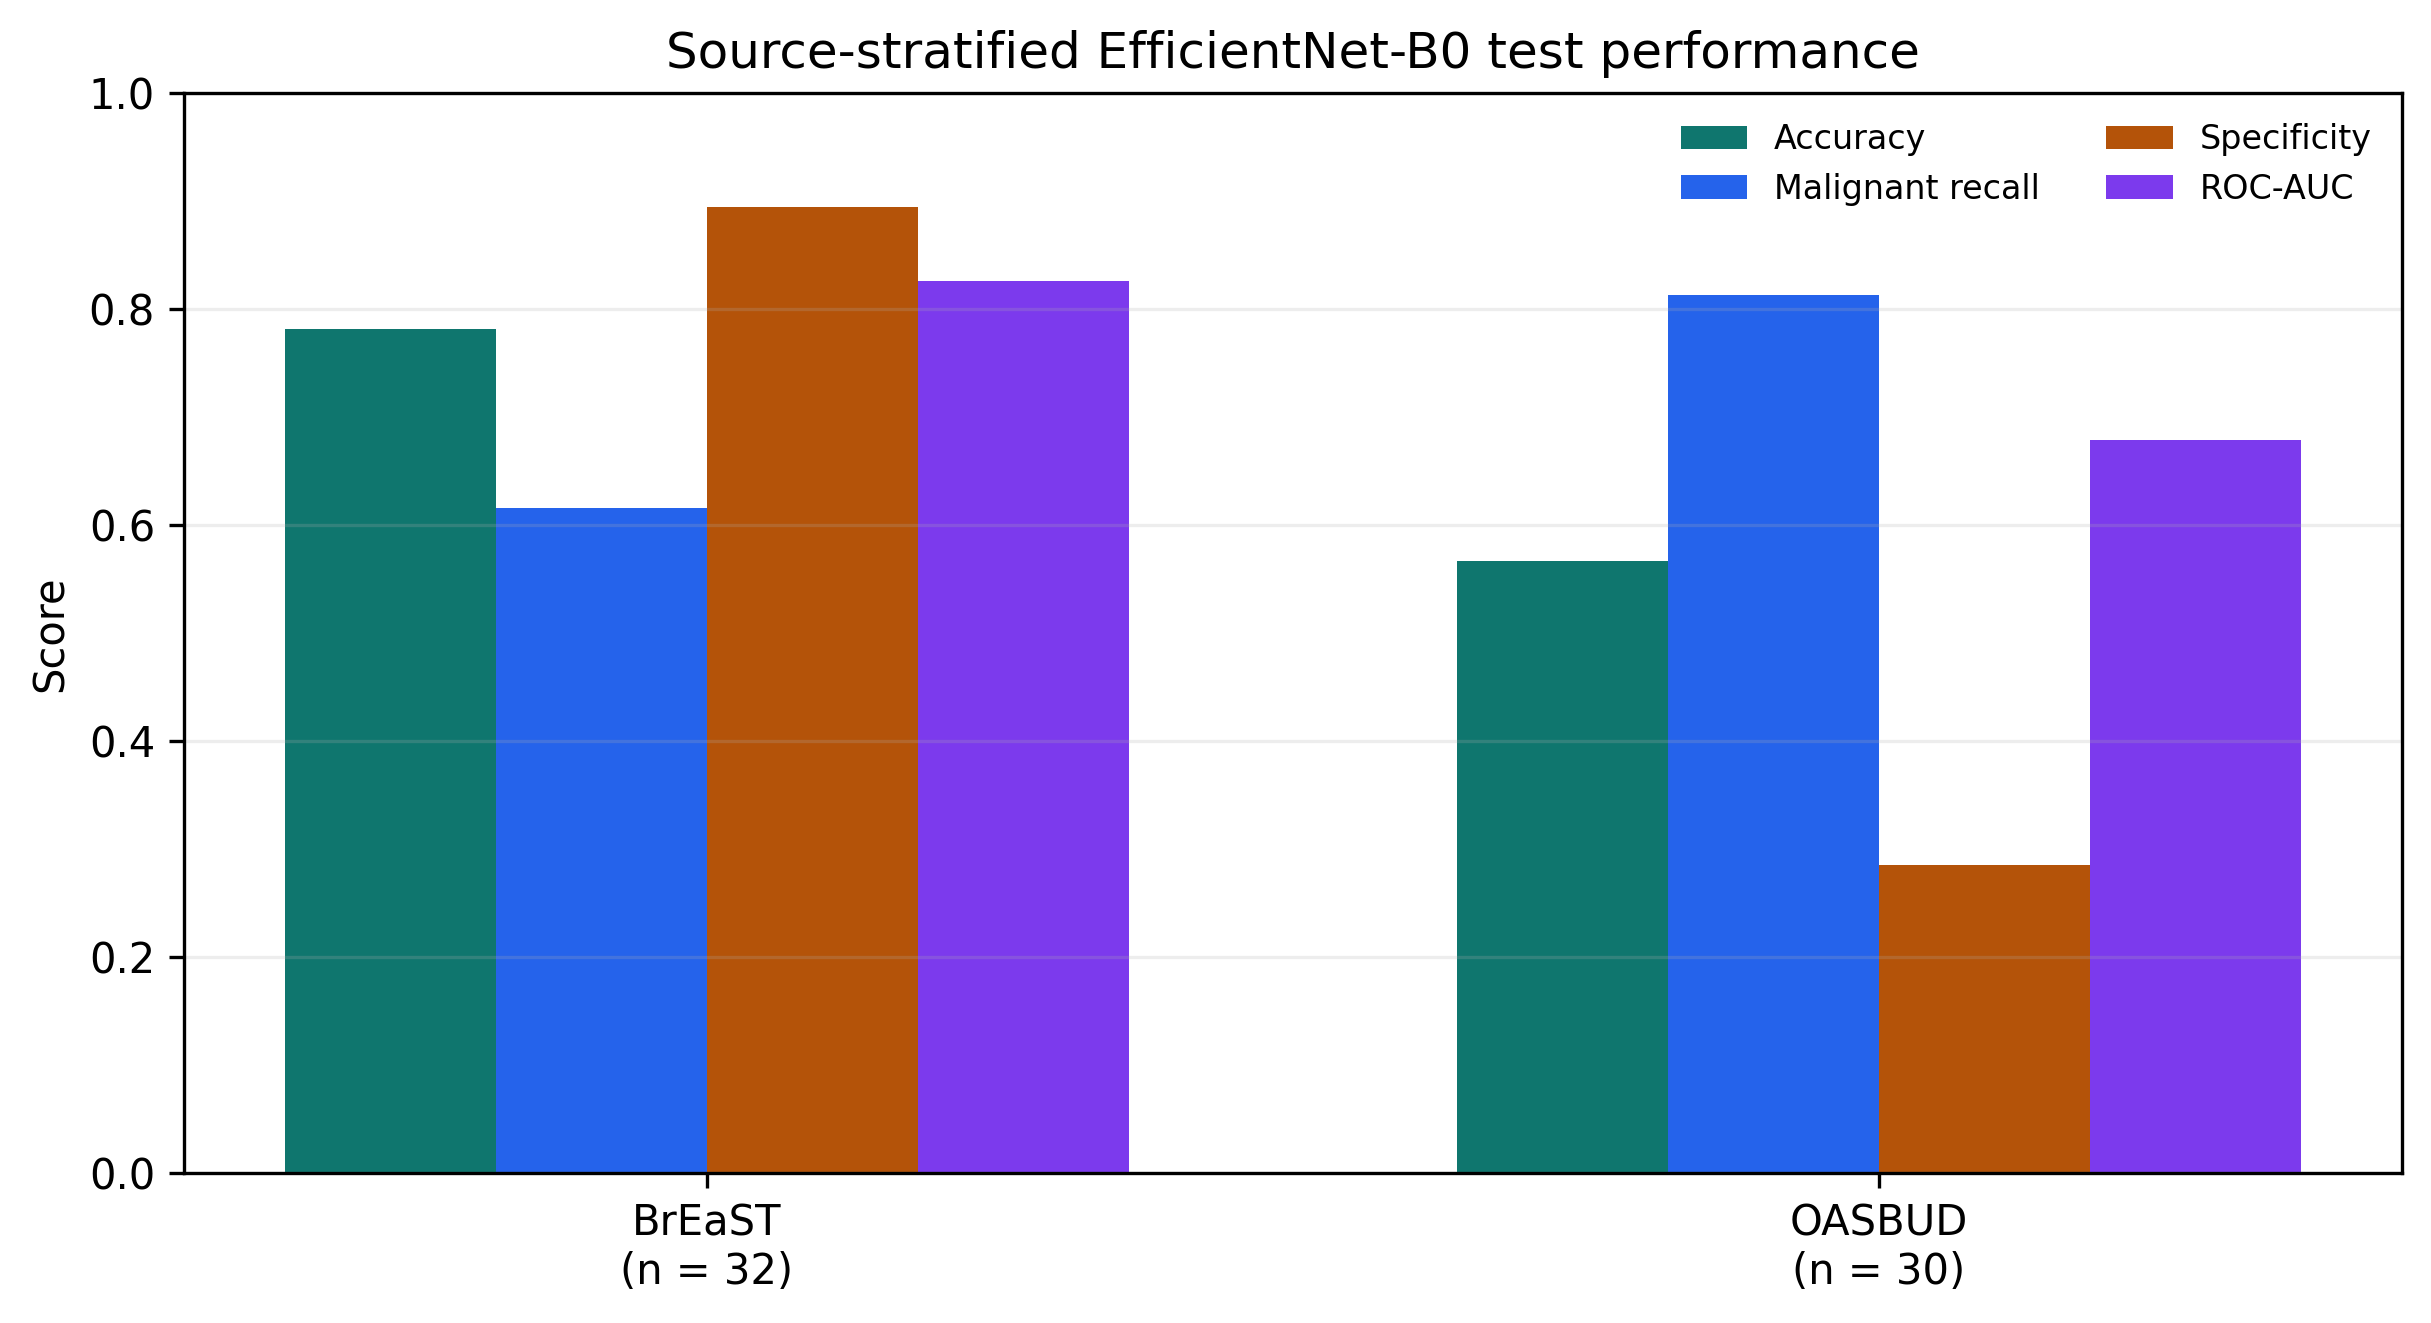
\includegraphics[width=0.92\textwidth]{figures/fig13_source_stratified_performance.png}
    \caption{Performance separated by source for the stored EfficientNet-B0 test predictions. This is an internal diagnostic of two small subsets, not external validation or a ranking of the source datasets.}
    \label{fig:source_results}
\end{figure}

OASBUD accounts for ten of the twelve false positives and three of the eight false negatives. BrEaST accounts for two false positives and five false negatives. The result suggests that a single pooled accuracy hides different error profiles. It does not show that one dataset is better, because source, case mix, reconstruction, lesion characteristics, and sample size are confounded. A larger protocol should report each source separately and predefine whether thresholds are shared or source-specific.

\section{Evidence status}
The most defensible result of this chapter is a clear evidence statement. The repository can execute a common preprocessing path, train three model families, produce machine-readable predictions, calculate metrics, and expose them through a local research interface. The audited local run yields the numerical results reported above. It does not establish external generalisation, clinical utility, superiority over published systems, or readiness for deployment.

\section{Reproducibility check}
The reported EfficientNet result was regenerated after the model-comparison run so that the primary metrics, confusion matrix, ROC curve, and per-image predictions refer to one checkpoint and one evaluation command. This matters because overlapping benchmark processes can otherwise leave a directory containing plots from one model and a metrics file from another. The final artefact set should always be inspected as a group before a value is copied into a table.

The current result is also intentionally modest in its wording. A 67.74\% accuracy on 62 local test images is evidence that the pipeline produced predictions above a chance-like baseline in this particular run; it is not evidence that the model will retain the same behaviour on new hospitals, devices, or patients. The confidence intervals and the audit caveat are therefore part of the result, not optional footnotes.

\section{Relationship to the original project narrative}
The submission-facing report removes historical values that could not be traced to a stored, audited experiment. This revision may appear less conclusive than an earlier narrative that described very high accuracy or simulated robustness curves. The change is deliberate. A dissertation should distinguish measured outcomes, planned experiments, and illustrative examples. Keeping those categories separate protects the reader and gives future work a clear starting point.

\section{Interpreting the custom CNN result}
The custom CNN achieved 64.52\% accuracy, macro F1 of 0.6452, and ROC-AUC of 0.6708, compared with 56.45\%, 0.5374, and 0.6364 for ResNet-50. In a small dataset, a simpler network can sometimes be easier to optimise and less prone to fitting incidental detail than a deeper transfer-learning model. That is a plausible explanation for this result, not a conclusion established by the current experiment. The accuracy intervals overlap: 0.5323--0.7581 for the custom CNN and 0.4355--0.6935 for ResNet-50. The data therefore support the statement that the custom CNN was the better-performing model in this run, while leaving the population-level ranking unresolved.

The result is still scientifically useful because it challenges the assumption that a larger or deeper model must win. It provides a concrete hypothesis for the next study: compare capacity, freezing strategy, and optimisation schedule across several seeds while holding the subject partition and tuning budget fixed. If the custom CNN remains competitive on a larger external cohort, that would be a meaningful engineering finding. It would still require clinical validation before any medical claim.
